We first present the 1-D shallow-water equations (SWE) for flood waves with variable bathymetry\cite{whitham1999_ch3}:

\begin{align*}
    h_t + (h v)_x &= 0 \\
    (h v)_t + \left[ hv^2 + \frac{1}{2} g h^2 \cos{(\alpha)} \right]_x &= g h \sin{(\alpha)} - C_f v^2
\end{align*}

where $v$ represents the average wave velocity, $h$ is the water depth, $C_f$ is a friction coefficient. Of these, $v$ 
and $h$ vary in time and space and $C_f$ and $\alpha$ may, in general, vary in space. For the scope of this project, we 
assume negligible friction so that $C_f$ is zero throughout. 

\begin{figure}[h]
    \centering
    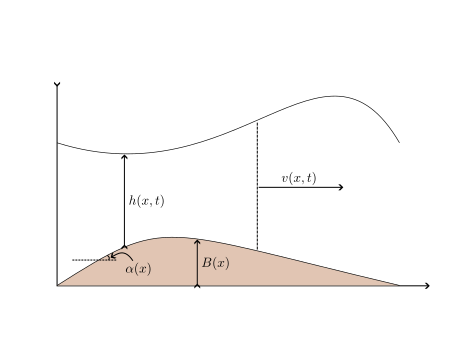
\includegraphics[width=0.8\textwidth]{images/swe_diagram.png}
    \caption{Shallow water scheme}
\end{figure}

\pagebreak
We expand the left-hand side of the second equation via the
chain rule and substitute $h_t = -h_x v - h v_x$ from the first equation to find: 

\begin{align*}
    (h v)_t + \left[ hv^2 + \frac{1}{2} g h^2 \cos{(\alpha)} \right]_x 
        &= \left( h_t v + h v_t \right) + h_x v^2 + 2 h v v_x + \left[ \frac{1}{2} g h^2 \cos{(\alpha)} \right]_x \\
        &= -h_x v^2 - h v v_x + h v_t + h_x v^2 + 2 h v v_x + \left[ \frac{1}{2} g h^2 \cos{(\alpha)} \right]_x \\
        &=  h v v_x + h v_t + \left[ \frac{1}{2} g h^2 \cos{(\alpha)} \right]_x \\
        &=  h \left( v v_x + v_t + g h_x \cos{(\alpha)} + \frac{1}{2} g h [\cos{(\alpha)}]_x \right) \\
        &=  h \left( v v_x + v_t + g h_x \cos{(\alpha)} + g h [\cos{(\alpha)}]_x - \frac{1}{2} g h [\cos{(\alpha)}]_x \right) \\
        &=  h \left( v_t + \left[ \frac{v^2}{2} + g h \cos{(\alpha)} \right]_x - \frac{1}{2} g h [\cos{(\alpha)}]_x \right).
\end{align*}

Hence we may express our system in conservation form as

$$
    \textbf{u}_t + \left[ F(\textbf{u}) \right]_x = S(\textbf{u})
$$

where (after dividing through by $h$)

$$
\textbf{u} = \begin{bmatrix}
    h \\
    v
\end{bmatrix}, \quad F(\textbf{u}) = \begin{bmatrix}
    hv \\
    \frac{v^2}{2} + g h \cos{(\alpha)}
\end{bmatrix}, \quad S(\textbf{u}) = \begin{bmatrix}
    0 \\
    g \sin{(\alpha)} - C_f \frac{v^2}{h} + \frac{1}{2} g h [\cos{(\alpha)}]_x
\end{bmatrix}.
$$

We expand $[F(\textbf{u})]_x$ to find:

$$
[F(\textbf{u})]_x = \begin{bmatrix}
    h v_x + h_x v \\
    v v_x + g h_x \cos{(\alpha)} + g h [\cos{(\alpha)}]_x
\end{bmatrix} = \begin{bmatrix}
    v                & h \\
    g \cos{(\alpha)} & v
\end{bmatrix} \begin{bmatrix}
    h \\
    v
\end{bmatrix}_x + \begin{bmatrix}
    0 \\
    g h [\cos{(\alpha)}]_x
\end{bmatrix}
$$

and so our system becomes

$$
\textbf{u}_t + A(\textbf{u}) \textbf{u}_x = \tilde{S}(\textbf{u})
$$

where 

$$
A = \begin{bmatrix}
    v                & h \\
    g \cos{(\alpha)} & v
\end{bmatrix}, \quad \tilde{S} = \begin{bmatrix}
    0 \\
    g \sin{(\alpha)} \left(1 + \frac{1}{2} h \alpha_x \right) - C_f \frac{v^2}{h}
\end{bmatrix}.
$$

When $\alpha = 0$ and frictional forces are negligible (i.e., $C_f = 0$), we recover the homogeneous system:

$$
A = \begin{bmatrix}
    v  & h \\
    g  & v
\end{bmatrix}, \quad \tilde{S} = \begin{bmatrix}
    0 \\
    0
\end{bmatrix}.
$$
